\chapter{\label{ch:least squares problem}Least Squares Problems}

\section{\label{sec:linear systems}Linear Systems}  %    S    S    S    S    S    S    S    S    S    S    S    S    S    S    S    S

  This story begins with the archetypal \index{matrix-vector equation} matrix--vector equation
  \begin{equation}   %  =   =   =   =   =
    \axeb .
    \label{eq:axeb}
  \end{equation}
The matrix $\A{}$ has $m$ rows, $n$ columns, and has rank $\rho$; the vector $b$ encodes $m$ measurements. The solution vector $x$ represents the $n$ free parameters in the model. In mathematical shorthand,
  \begin{equation}   %  =   =   =   =   =
    \aicmnr, \quad b \in \cmplxm, \quad x \in \cmplxn
  \label{eq:basics}
  \end{equation}
with $\cmplx{}$ representing the field of complex numbers. The matrix $\A{}$ and the vector $b$ are given, and the task is to find the vector $x$.

\subsection{\label{ssec:exact soln}Exact Solution}  %   SS   SS   SS   SS   SS   SS   SS   SS   SS   SS   SS   SS
The letters in \eqref{eq:axeb} will change, but the operation remains the same: a matrix operates on an $n-$vector and returns an $m-$vector. We can think of the \index{matrix} matrix as a map from vectors of dimension $n$ to vectors of dimension $m$:
  \begin{equation*}   %  =   =   =   =   =
    \A{} \colon \cmplxn \mapsto \cmplxm .
  \end{equation*}

If the vector $b$ can be expressed a combination of the columns of the matrix $\A{}$ then there is a direct solution:
%  e q u a t i o n
\begin{equation*}
  %\begin{split}
    \axeb \quad \Longrightarrow \quad x_{1} a_{1} + \cdots + x_{n} a_{n} = b
  %\end{split}
%\label{eq:}
\end{equation*}
%  e q u a t i o n
and the residual error \index{residual error} vanishes:
  \begin{equation*}   %  =   =   =   =   =
   %\begin{split}
      \axmb = \zero
   %\end{split}
 %\label{eq:}
  \end{equation*}
where the zero vector $\zero$ is a list of $m$ zeros. The total error, the norm of this vector, is 0.

For example, for the problem where the system matrix $\A{}$ is the identity matrix $\I{2}$:
  \begin{equation*}   %  =   =   =   =   =
   %\begin{split}
      \idtwo \xtwo = \mat{c}{b_{1} \\ b_{2}}
   %\end{split}
 %\label{eq:}
  \end{equation*}
The solution is
  \begin{equation*}   %  =   =   =   =   =
   %\begin{split}
      \xtwo = \mat{c}{b_{1} \\ b_{2}} .
   %\end{split}
 %\label{eq:}
  \end{equation*}
There is no residual error 
  \begin{equation*}   %  =   =   =   =   =
   %\begin{split}
      \A{} x - b = \zerotwo .
   %\end{split}
 %\label{eq:}
  \end{equation*}

\subsection{\label{ssec:no exact soln}No Exact Solution}  %   SS   SS   SS   SS   SS   SS   SS   SS   SS   SS   SS   SS
But what happens when the vector $b$ is \emph{not} in the column space of the matrix $\A{}$? We must relax our solution criteria and instead of insisting upon zero residual error, we ask for minimal residual error. Instead of a perfect solution, we ask for the best solution. One such class of solutions are least squares solutions\index{leasts squares!solutions}.

To demonstrate this point, the previous example is modified to be:
  \begin{equation*}   %  =   =   =   =   =
      \mat{cc}{1 & 0 \\ 0 & 0} \xtwo = \mat{c}{b_{1} \\ b_{2}} .
  \end{equation*}
When $b_{2} \ne 0$ there is no exact solution. Consider the solutions given by
  \begin{equation}   %  =   =   =   =   =
      x_{*} = \mat{c}{ x_{1} \\ 0 } .
      \label{eq:xstar}
  \end{equation}
The error is 
  \begin{equation*}   %  =   =   =   =   =
   %\begin{split}
      \A{} x - b = -\mat{c}{0 \\ b_{2}}
   %\end{split}
 %\label{eq:}
  \end{equation*}
which has a norm of $b_{2}$. This is the least possible error for the problem and we can safely call \eqref{eq:xstar} the best solution. In this light, the transition from an exact solution to an inexact solution is natural.

There are two fundamental types of least squares solutions of interest and they are classified by the interpretation of the output. In the first case, zonal approximation, the output represents data at a physical zone, a point or a region. In the second case, the output represents an amplitude, a contribution for a mode. Basic examples follow.

\subsection{\label{ssec:zonal approx}Zonal Approximation}  %   SS   SS   SS   SS   SS   SS   SS   SS   SS   SS   SS   SS
Consider the vector field $F$ described by the gradient of a scalar field $\phi$.
  \begin{equation*}   %  =   =   =   =   =
    F = \nabla \phi
  \end{equation*}
In practice one measures the vector field and solves the inverse problem. The input and outputs are represented in \ref{fig:sticks}. The physical field is $\phi(x)$, $0\le x \le 2$, the approximation is $\varphi_{x_{k}}$, $k=0,1,2$. For a cleaner presentation let $\varphi_{x_{k}} \rightarrow \varphi_{k}$. The first measurement $x_{1}$ represents the potential change between $\phi(0)$ and $\phi(1)$; the second measurement $x_{2}$ the change between $\phi(1)$ and $\phi(2)$.
  \begin{equation*}   %  =   =   =   =   =
    \begin{split}
      \varphi_{1} - \varphi_{0} &\approx \delta_{1} \\
      \varphi_{2} - \varphi_{1} &\approx \delta_{2}
    %\label{eq:}
    \end{split}
  \end{equation*}
\begin{figure}[htbp] %  figure placement: here, top, bottom, or page
   \centering
   \includegraphics[ width = 3in ]{../"ells graphics"/"least squares"/"sticks 04"} 
   \caption[Scalar function $\phi$ and approximations.]{Scalar function $\phi(x)$ (curve) and approximation $\varphi_{k}$ (sticks).}
   \label{fig:sticks}
\end{figure}

The system matrix 
  \begin{equation*}   %  =   =   =   =   =
   %\begin{split}
      \A{} =     \mat{rrr}{ 
      -1 & 1 & 0 \\
       0 & -1 & 1 } \in \real{2 \times 3}_{2}.
   %\end{split}
 %\label{eq:}
  \end{equation*}
There are $m = 2$ measurements, $n = 3$ measurement locations, and the matrix rank is $\rho = 2$. Because the rank is less than the number of columns, $\rho < n$, this problem is \emph{underdetermined} \index{underdetermined system}.

The linear system is
  \begin{equation}   %  =   =   =   =   =
    \mat{rrr}{ 
      -1 & 1 & 0 \\
       0 & -1 & 1 }
    \mat{c}{ \varphi_{0} \\ \varphi_{1} \\ \varphi_{2} }
    =
    \mat{c}{ \delta_{1} \\ \delta_{2} } .
    \label{eq:zonalls}
  %\end{split}
  \end{equation}

\subsection{\label{ssec:modal approx}Modal Approximation}  %   SS   SS   SS   SS   SS   SS   SS   SS   SS   SS   SS   SS
In the modal approximation, the user first selects a set of basis functions to describe measurements. Popular basis functions include orthogonal polynomials, trigonometric functions, or monomials. For example, a linear regression implies a basis set of two elements: a constant function, and a linear function. This leads to the familiar equation for a straight line:
  \begin{equation*}   %  =   =   =   =   =
    y(x) = a_{0} + a_{1} x
  \end{equation*}
The $n=2$ parameters represent the intercept $\paren{a_{0}}$, and the slope $\paren{a_{1}}$. Each of the $m$ measurements represents the straight line:
  \begin{equation*}   %  =   =   =   =   =
   \begin{split}
     a_{0} + a_{1} x_{1} &= y_{1} \\
       & \ \, \vdots \\
     a_{0} + a_{1} x_{m} &= y_{m} .
    %\label{eq:}
   \end{split}
  \end{equation*}

Taken together, the measurements compose the system
  \begin{equation}   %  =   =   =   =   =
   \begin{split}
     \mat{cc}{ 1 & x_{1} \\ \vdots & \vdots \\ 1 & x_{m} }
     \mat{c}{ a_{0} \\ a_{1} }
     =
     \mat{c}{ y_{1} \\ \vdots \\ y_{m} }
    \label{eq:modalls}
   \end{split}
  \end{equation}

\section{\label{sec:lss}Least Squares Solutions}  %    S    S    S    S    S    S    S    S    S    S    S    S    S    S
In both the zonal and modal approximations, there is exact solution and we to minimize the residual error
  \begin{equation*}   %  =   =   =   =   =
   %\begin{split}
      \norm{\axmb}.
   %\end{split}
 %\label{eq:}
  \end{equation*}
This work explores the minimal solutions under the $2-$norm, the familiar norm of Pythagorus:
  \begin{equation*}   %  =   =   =   =   =
   %\begin{split}
      \normt{ \mat{c}{x_{1} \\ x_{2}} } = \sqrt{x_{1}^{2} + x_{2}^{2}}.
   %\end{split}
 %\label{eq:}
  \end{equation*}


\subsection{\label{ssec:zonal solution}Zonal Solution}  %   SS   SS   SS   SS   SS   SS   SS   SS   SS   SS   SS   SS

The solutions for the linear system in \eqref{eq:zonalls} which minimize $\normt{\axmb}$ are
  \begin{equation*}   %  =   =   =   =   =
    \mat{c}{ \varphi_{0} \\ \varphi_{1} \\ \varphi_{2} } =
    \mat{rr}{ -2 & -1 \\ 1 & -1 \\  1 & 2 }
    \mat{c}{ \delta_{1} \\ \delta_{2} } + \alpha
    \mat{c}{ 1 \\ 1 \\ 1 }, \qquad \alpha \in \cmplx{} .
  \end{equation*}
There is a continuum of solutions due to the fact that
  \begin{equation*}   %  =   =   =   =   =
    \Ax = \A{} \paren{x + \alpha \mat{c}{ 1 \\ 1 \\ 1 } } .
  \end{equation*}
An easy demonstration is to write
  \begin{equation*}   %  =   =   =   =   =
    \A{} \mat{c}{ 1 \\ 1 \\ 1 } 
      = \mat{rrr}{ -1 & 1 & 0 \\ 0 & -1 & 1 } \mat{c}{ 1 \\ 1 \\ 1 } 
      = \mat{c}{ 0 \\ 0 } .
  \end{equation*}

\subsection{\label{ssec:modal solution}Modal Solution}  %   SS   SS   SS   SS   SS   SS   SS   SS   SS   SS   SS   SS
The linear system is \eqref{eq:modalls} can be case using the column vectors
  \begin{equation*}   %  =   =   =   =   =
   \begin{split}
     {\bf{1}} = \mat{cc}{ 1 \\ \vdots \\ 1 }, \quad
     x = \mat{cc}{ x_{1} \\ \vdots \\ x_{m} }, \quad
     y = \mat{cc}{ y_{1} \\ \vdots \\ y_{m} } .
    %\label{eq:}
   \end{split}
  \end{equation*}
The columns of the system matrix $\A{} = \mat{c|c}{\bf{1} & x}$. The solution parameters can be expressed in terms of the column vectors:
  % = =  e q u a t i o n
  \begin{equation*}
    \mat{c}{\alpha_{0} \\ \alpha_{1}} =
    \paren{ \paren{\oto}\paren{\xtx} - \paren{\otx}^{2}}^{-1}
    \mat{rr}{\xtx & -\otx \\
            -\otx &  \oto }
    \mat{c}{ \mathbf{1}^\mathrm{T}y \\  x^\mathrm{T}y} .
  \end{equation*}
  % = =

\section{\label{sec:lsp}Least Squares Problem}  %    S    S    S    S    S    S    S    S    S    S    S    S    S    S    S    S
Emboldened by solutions to two basic problems, we turn attention towards formalities. Starting with a the linear system $\axeb$ where the matrix $\aicmn$, the data vector $b\in\cmplxm$, the least squares solution\index{least squares!solution!definition} $x_{LS}$ is defined as the set
  \begin{equation}   %  =   =   =   =   =
    \xlsdef .
  \end{equation}
The least squares solution may be a point or it may be a hyperplane. A general solution is
  \begin{equation*}   %  =   =   =   =   =
    x_{LS} = \solnls{b}{y}, \qquad y \in \cmplx{n}
  \end{equation*}
where the matrix $\Ap$ is the pseudoinverse.

\section{\label{sec:ftola}Fundamental Theorem of Linear Algebra}  %    S    S    S    S    S    S    S    S    S    S    S    S    S    S    S    S
  \begin{table}[htbp]  %  T A B L E
    \caption[The Fundamental Theorem of Linear Algebra]{\index{Fundamental Theorem of Linear Algebra!orthogonal decomposition}The Fundamental Theorem of Linear Algebra for $\aicmn$ }
    \begin{center}
    		\begin{tabular}{rlcccccccc}
    		  %
    		  domain:   & $\cmplx{n}$ & = & $\brnga{*}$ & $\oplus$ & $\rnlla{}$ \\
    		  %
    		  codomain: & $\cmplx{m}$ & = & $\brnga{}$  & $\oplus$ & $\rnlla{*}$
    		  %
      \end{tabular}
    \end{center}
  \label{tab:ftola}
  \end{table}%

  \begin{table}[ht]
    \caption[The Fundamental Theorem of Linear Algebra in pictures]{The Fundamental Theorem of Linear Algebra for $\aicmn$}
    \begin{center}
      \begin{tabular}{crclc}
          %
          Domain &&&& Codomain \\\hline
          %
          \ \\
          %
          $\cmplxn$ &&&& $\cmplxm$ \\[10pt]
          %
          \multirow{3}{*}{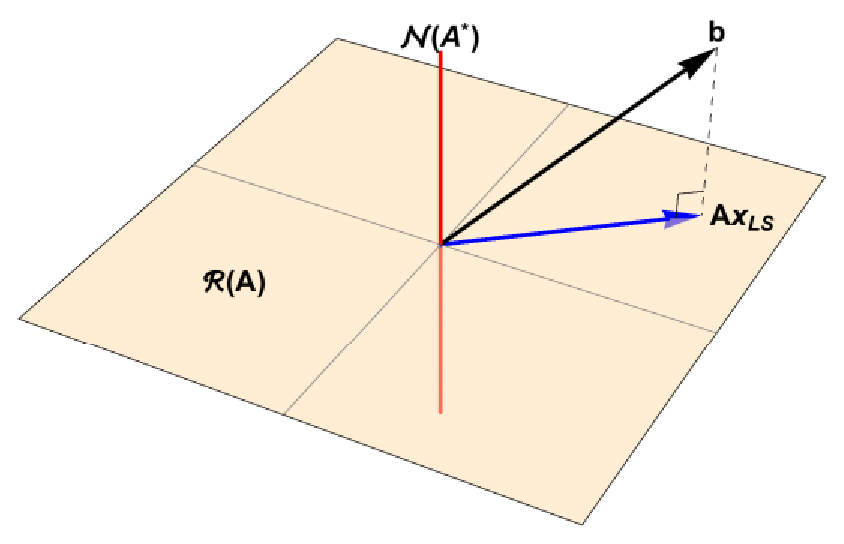
\includegraphics[ width = 1.7in ]{../graphics/ftola/domaingimp}} &&&&
          \multirow{3}{*}{\includegraphics[ width = 1.7in ]{../graphics/ftola/codomaingimp}} \\[5pt]
            & $\A{} \colon \cmplx{n}$ & $\mapsto$ & $\cmplx{m} $ \\[15pt] 
            & $\cmplx{n}$ & $\mapsfrom$ & $\cmplx{m} \colon \A{*}$ \\
          %
      \end{tabular}
    \end{center}
  \end{table}

